\documentclass{master_thesis}
\addbibresource{refs.bib}

\begin{document}
\section{Case study}

% \subsection{Steps}
Steps
\begin{enumerate}
	\item Set up automates accessibility issue detection in storybook
	adding a11y-addon + find a way to generate report of all issues. \\
	\textbf{Data gathered from automated testing report:}
	\begin{itemize}
		\item How many occurrences in the accessibility violations report. This will show how many violations where detected from all the examples. Might contain the same issue multiple times.
		\item How many unique issues will only count different violations for each component.
		\item How many passed checks – this together with violations will show how many things where tested for each component – Most component have more than one story – the list will contain all different passed checks listed
		\item How many valid checks – are the passed checks relevant to the component – only count the ones that are related to the component that the example is about.
	\end{itemize}
	\item Manual accessibility audit with other team members. We already had the add-on set up, and we used storybook preview of components for testing, so we looked at the violations reported by the addon-a11y also.
	\item Comparison between manual and automated report
	\item Research other possibilities. Testing new storybook test-runner to automatically run all a11y tests. How can we ignore some issues without losing the info.
	\item Set up a new solution in a new component library. Will it help to ensure better accessibility from the beginning?
\end{enumerate}

Pipedrive has been developing a sales CRM using mostly typescript and React. Accessibility has never been high priority and at this point it is not very easy to get started. We have a design system and a React based component library to keep the look and UX consistent. This seems like a good place to start with solving accessibility issues. The library is used widely in the company and developer from different teams contribute to it. If a button in the reusable library gets fixed 95\% of the buttons in the web app that our customers use should be improved.

This should not be taken as a way to solve all accessibility problems, but a good first step to get started. Making changes in a reusable UI library should have a wide impact on the products overall accessibility and without reaching some basic level there first it could be hard to start testing views in the final product.

\subsection{Current state of awareness about accessibility in the company}

First I sent out a survey in our company Slack channels (see figure \ref{fig:slack-message}) to understand what is the knowledge and general approach on web accessibility in the company. It was shared in one front end developers channel with 212 members, designers channel with 73 members, accessibility channel with 31 members and in out component library channel with 124 members. Some people might also be in more than one of these channels. The aim was to reach people in the company who would be most likely to be using these tools and who would be likely contributors to the library. There were 7 questions and some of they also included a field for free text to give more details on the subject if they wanted.

In total 20 people replied to the survey - 6 designers and 14 developers, including one engineering manager. This does not give a full overview of the company, but it should give a good insight into what general opinions regarding accessibility might be. It is likely that developers and designers that are more involved with our component library and/or interested in accessibility where more likely to respond.

The results show that 10\% of people who responded think their knowledge on accessibility is very good, while most think that knowledge level is average. 35\% of responders know where do find resources about accessibility standards, 15\% don't know and 50\% know, but think they need more. They don't see that accessibility has high priority in the company currently, but at the same time 40\% of responders think that following accessibility standards should be prioritized. There were several comments in the free text sections expressing saying they appreciate this subject being opened.

\subsection{Adding tests to our component library}
The next step was adding some automated test to our component library development workflow and observing their usefulness. The aim was to find something that we can integrate to our development workflow without a need to learn a new tool or add unnecessary complexity.

We use Storybook for our UI development. It is an open source software for UI development tool that allows you to work on one component at a time \citep{storybook}. It allows us to render isolated UI components without integrating them to the final product right away. Our developers use it to test out the components they are developing locally. We also have a version of storybook available for anyone in the company to see with all the components. If this is the first place where elements will be rendered it seems logical to try to find a way to start testing them there.

To show a component you need to write a story - this means use it the way you would use it in the real world, and it will be rendered in a browser inside Storybook UI. It also has a sidebar for navigating between different examples, controls for additional tools and documentation. This means using a browser extension for accessibility tests would also test the UI around the actual example.

Storybook has a wide ecosystem of add-ons and one of them is addon-a11y. It uses Deque's axe-core to audit the html rendered for an isolated component \citep{addon-a11y}. Axe is an accessibility testing engine for websites and other HTML-based user interfaces. It includes WCAG 2.0 and 2.1 on level A and AA and promises to catch 57\% of WCAG issues on average. \citep{Deque2023} This should be taken with a grain of salt, because we are intending to test isolated element and not the whole webpage and other studies comparing accessibility testing tools effectiveness have found the coverage to be lower  \todo{{needs citation}}.
This seemed like the best solution in our situation so addon-a11y was added to our component library's storybook. The tool is visible in the sidebar of every example. It shows all the checks that it has passed, all the violations that where found and any issues that could not be checked and might need manual testing. Every rule listed there also has reference to the html node that had the violation, explanation and links to Deque webpage with examples. This should be very useful in understanding and fixing these issues.
It does not generate a report of all the issues found across the whole library for this another tool was used that will go through all the examples and generate a summary of all the violations found.

% During the time of this testing axe-core improved in evaluating color contrast for disabled elements. At the time of the audit they were evaluated for color contrast issues, but later this has been improved to comply with the change in WCAG standard.\\
% The issue with Modals, dialogs and similar elements is that they never get checked. Could we improve this by changing the examples provided in storybook.

\subsection{Manual accessibility audit}

The second part is conducting a manual accessibility audit in the same library and comparing the results with the automatically generated test report results to determine what are its strengths and weaknesses and if testing isolated components poses any limitations.
\subsubsection{Methodology for manual audit}
In order to look at each component in isolation we used storybook here too. The accessibility add-on had already been installed and we looked at the violations reported there too. We worked in a team of 4 people - 3 designers and 1 developer. We created a task for each component - 53 tasks in total.

We checked violations in accessibility add-on panel (see figure \todo{add figure}), tried using only a keyboard to navigate, tried using a screen reader to navigate. Each component had 1 or more examples. As many as was relevant to get the whole picture where looked at.

In the beginning of the audit we tested an add-on in storybook for mocking a screen reader (\todo{Refeence for this add-on and maybe and article about the difficulty of using a screen reader}). It had the option to show the output a normal screen reader would play as audio as text. Initially it seemed like convenient solution with rather reliable results, but further investigation revealed that the output was very different from what an actual screen readers. For the rest on the audit we used Voice over - the MacBook built in screen reader, because it was available to us. There was and initial learning curve, but after that it went quite smoothly. All the component that had already been tested with the faulty add-on where looked over again using Voice over.

The audit results where documented in a table. We approached the problems for the users perspective and looked at what issues different types of users might encounter. We separated them to 3 sections:
\begin{enumerate}
	\item Mouse user issues
	\item Keyboard user issues
	\item Screen reader user issues
\end{enumerate}

We see this separation as a good way to prioritize  fixing the issues in the future. Mouse user is the user we are considering in all of our development currently. The issues they would encounter should be most critical. This category includes a lot of visual, color contrast and image text issues.

The second type of user would encounter all the issues from the first category plus everything that is unreachable to them by using a keyboard. We looked at what functionality is or should be working when you use a mouse and tried to do the same things by only using a keyboard.

The third user was imitated by using a screen reader. The prerequisite for this was keyboard usability - if it was not possible to navigate using a keyboard then most likely it would not be very usable by a screen reader.

In real life these users might not be so clearly separated and there were many issues that would affect all types of users, but as the intention was to come out of the audit with an actionable list we needed to prioritize the issues while we found them in order of severity and current customer impact. These categories also mostly depend on each other, so it would make sense in most cases to start from solving mouse user issues, then keyboard user issues and then screen reader user issues.

\subsubsection{Comparing results from manual audit and automated report}

To get the whole list including all components a report was created that included the violations caught in each example of each component. This report was generated at the beginning of the manual audit, so the results obtained from both methods are based on the same source code.

\todo{fix charts}
I prepared a comparison table form both results. For automated accessibility tests I recorded the number of examples that included violations, the number of different violations and the number of passed checks for each component. In most cases there were more examples with violations because the same thing was reported in more than one example (see figure \ref{fig:audit-fail} \todo{fix chart}). Passed issues where looked over to determine how many where valid to the isolated component (see figure \ref{fig:audit-pass}\todo{fix chart}).
\begin{figure}[h]
	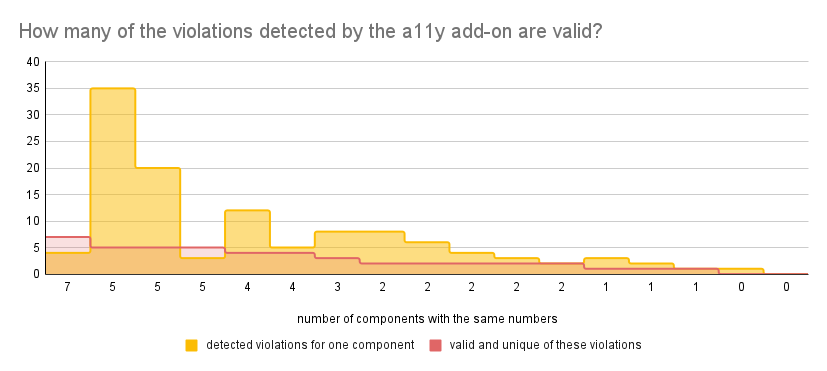
\includegraphics[width=\textwidth]{img/audit_violations.png}
	\caption{Number of violations detected by a11y add-on and how many of them are valid}
	\label{fig:audit-fail}
\end{figure}
\begin{figure}[h]
	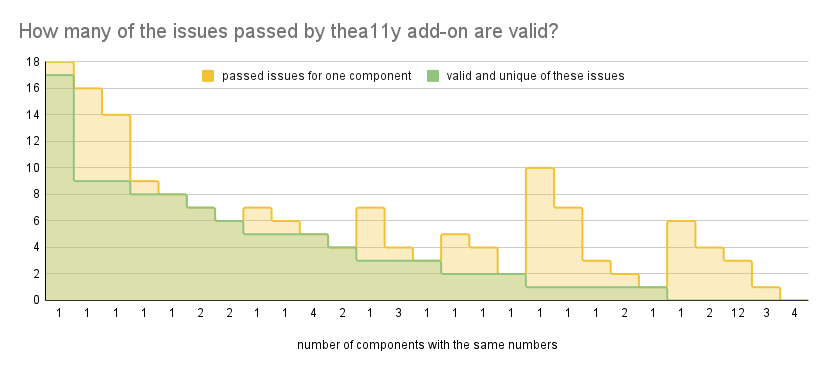
\includegraphics[width=\textwidth]{img/audit_passed.png}
	\caption{Number of passed issues detected by a11y add-on and how many of them are valid}
	\label{fig:audit-pass}
\end{figure}

In some cases there were 0 violations detected, and 0 valid checks passed – this means that the automated testing was not effective (\todo{Make chart or table for this}).

\subsubsection{Limitations of using Storybook's addon-a11y}

The accessibility add-on in Storybook analyzes the examples that have been made for the component and unsuitable example can cause false results. Items that are triggered by another element, like modals and popups are currently in our library displayed with a button as a trigger. The initial html that the accessibility tests are run on only has the button and the tests are not being run again after triggering the element. This could potentially be remedied with better examples.

The biggest limitation of this tool currently is that it can only be view-d in storybook. To see the number of passes and fails you need to open the accessibility tab for each component. I looked into ways of automating this so that the same checks could be run on every change to the library and added to continuous integration (CI) workflow. In the current version of Storybook there is no easy way to do this, but it will become much easier in the next major version.

Upgrading out component library to that version need some extra work to make it compatible, but I have tested out this solution on a test library, and it seems like it would definitely be an improvement. Running the tests in CI would ensure that they are run every time someone makes a change and not only when we choose to. We could also block changes that don't pass the required accessibility checks.

\todo{Reasons for automated check not being effective}
\todo{fix charts}
\todo{Generated charts/ tables with these numbers - component}

\end{document}